To evaluate the applicability of machine learning techniques for secondary reserve allocation the study was conducted using the Spanish electricity market historical data.

\subsection{Data Sources and Preprocessing}

The case study utilizes publicly available operational and historical data from the Spanish \gls{TSO}, \gls{REE} (please check the Data Availability Statement). The dataset includes the key variables presented in Table~\ref{esios_data}.

\begin{table}[H] 
\caption{This is a table caption. Tables should be placed in the main text near to the first time they are~cited.\label{tab1}}
\newcolumntype{C}{>{\centering\arraybackslash}X}
\begin{tabularx}{\textwidth}{CCCC}
\toprule
\textbf{ESIOS Code}	& \textbf{ESIOS Name} & \textbf{Variable}	& \textbf{Units}\\
\midrule
632 & Secondary Reserve Allocation AUpward     & Up Allocated & MW\\
633 & Secondary Reserve Allocation ADownward   & Down Allocated & MW\\
680 & Upward Used Secondary Reserve Energy  & Up Used & MWh\\
681 & Downward Used Secondary Reserve Energy    & Down Used & MWh\\
1777    & Wind D+1 Daily Forecast  & DA Wind & MWh\\
1779    & Photovoltaic D+1 Daily Forecast  & DA PV & MWh\\
1775    & Demand D+1 Daily Forecast    & DA Demand & MWh\\
10258   & Total Base Daily Operating Schedule PBF Generation  & DA Schedule Generation & MWh\\
14  & Base Daily Operating Schedule PBF Solar PV  & DA Schedule PV Generation  & MWh\\
10073   & Base Daily Operating Schedule PBF Wind     & DA Schedule Wind Generation & MWh\\
10186   & Base Daily Operating Shedule PBF Total Balance Interconnections  &   DA Scheduled Tie Lines & MWh\\
\bottomrule
\end{tabularx}
% \noindent{\footnotesize{\textsuperscript{1} Tables may have a footer.}}
\end{table}


The data spans multiple years to account for seasonal variability and long-term trends in vRES generation and demand. Data preprocessing only handled missing values using interpolation methods, with IterativeImputer \cite{vanBuuren2011,Buck1960}, as presented in Figure~\ref{fig:misisng_data}.

\begin{figure}[H]
    \centering
    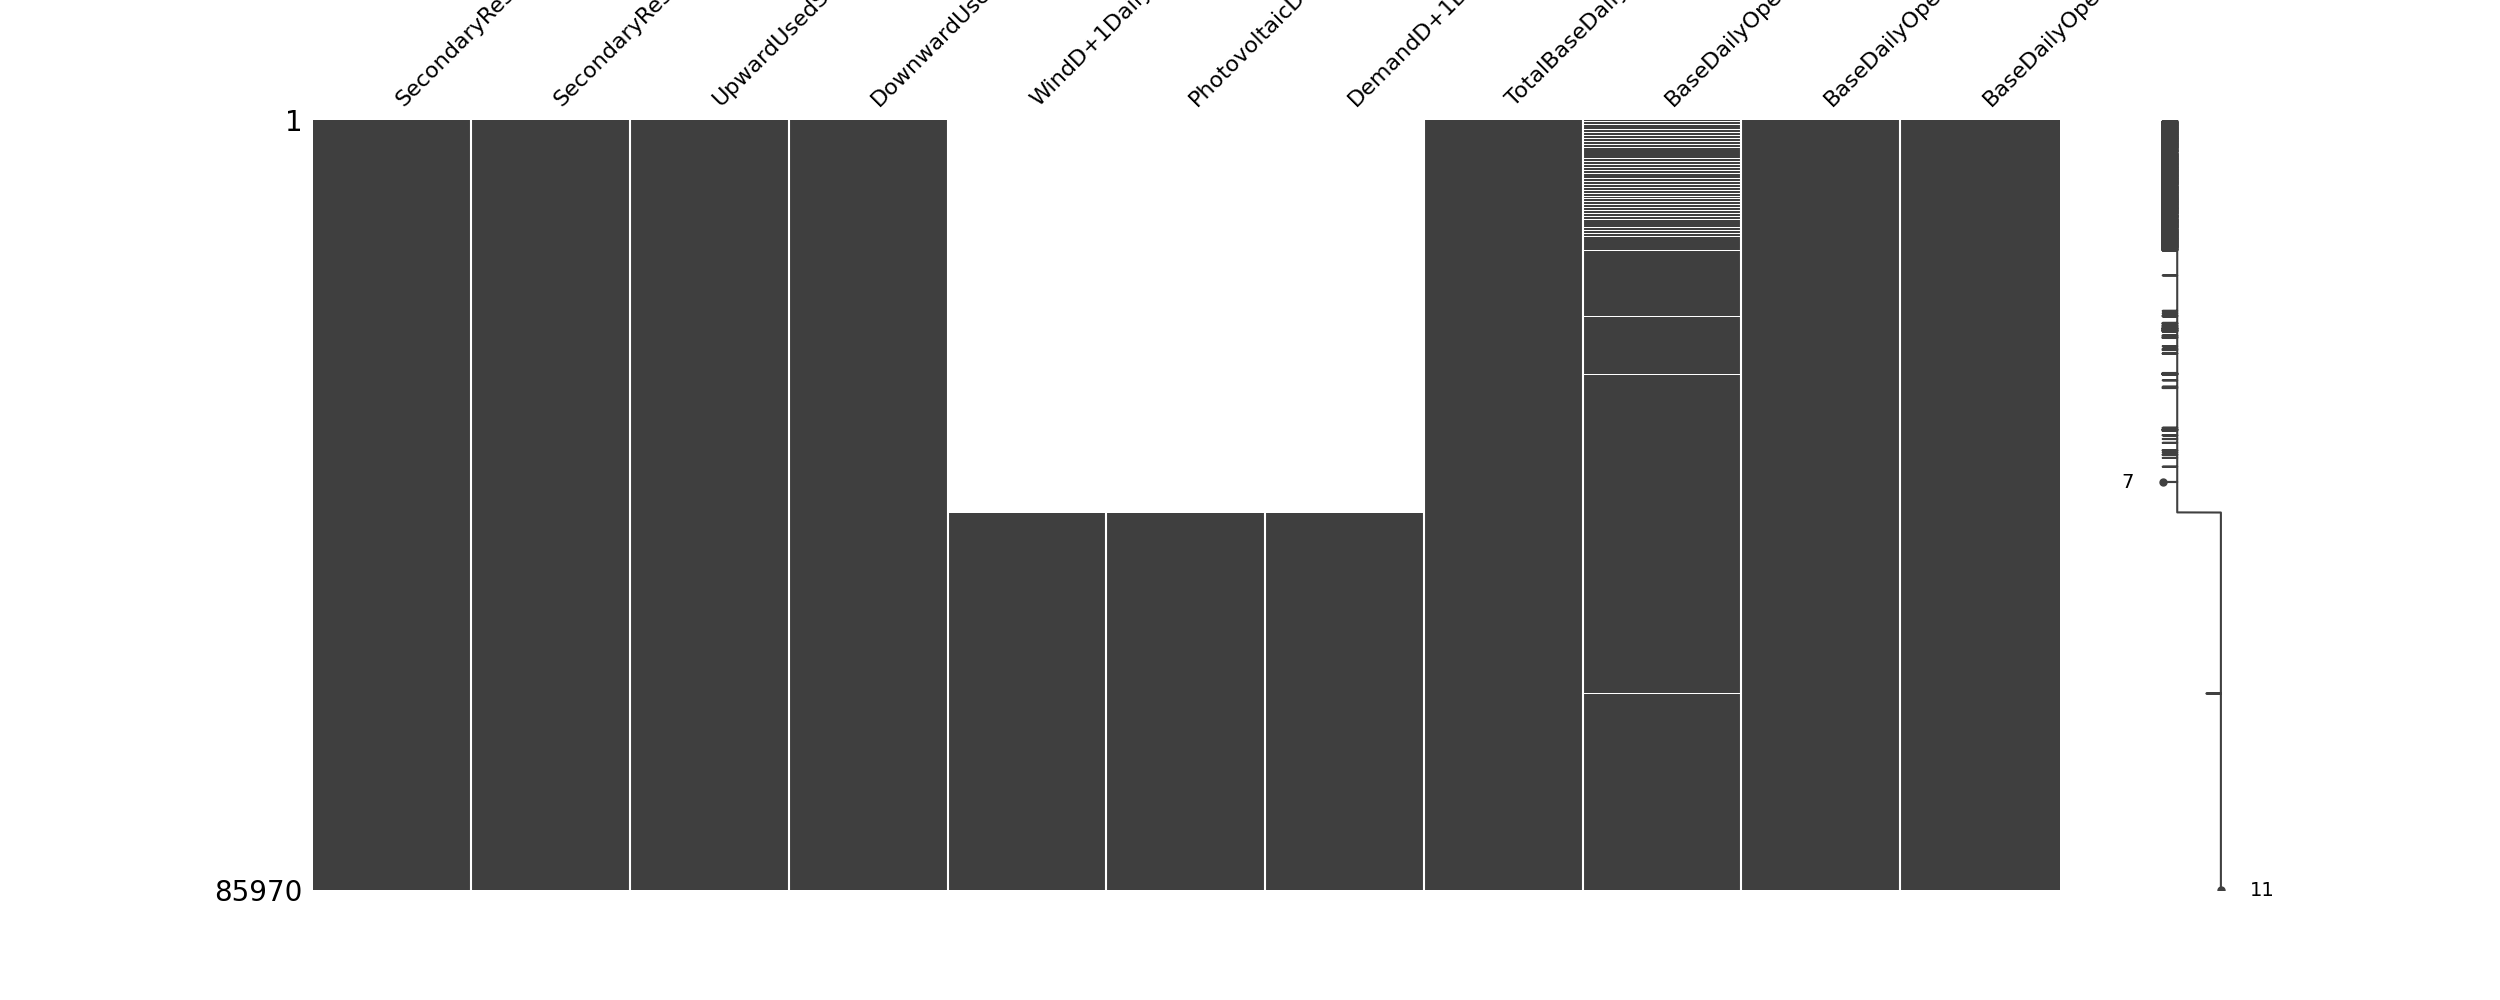
\includegraphics[width=\textwidth]{plots/missing_data.png}
    \caption{Missing Data.}
    \label{fig:misisng_data}
  \end{figure}
	

To choose the temporal space of the models temporal auto-correlations were checked in Table~\ref{temp_corr}.

\begin{tabular}{lllllllllll}
\toprule
\midrule
\multirow[t]{2}{*}{UpwardUsedSecondaryReserveEnergy} & horas & 1 & 2 & 24 & 23 & 25 & 168 & 144 & 192 & 48 \\
 & rácio & 0.44 & 0.24 & 0.22 & 0.19 & 0.19 & 0.17 & 0.16 & 0.16 & 0.16 \\
\cline{1-11}
\multirow[t]{2}{*}{DownwardUsedSecondaryReserveEnergy} & horas & 1 & 2 & 24 & 23 & 25 & 168 & 144 & 192 & 48 \\
 & rácio & 0.43 & 0.22 & 0.25 & 0.20 & 0.19 & 0.21 & 0.19 & 0.20 & 0.19 \\
\cline{1-11}
\bottomrule
\end{tabular}


From Table~\ref{temp_corr} can be verified the small correlation between variables,  

The goal is to forecast \gls{DA} values 24 hours ahead. As for the input for that forecast the temporal correlations present 168 hours as the next correlation after the one day period, which represents a week.
Variables has been added to account for each time range: day, day of year, month, day of week.\par
So, models will receive data in (Batch Size, 168, 18) shape for input, and (Batch Size, 24, 1) shape for output.



\subsubsection{Training Data}
For training the full dataset from 2014 to 2023, the data used has the following metric presented in Table~\ref{training_data_sum}:

\begin{table}[H] 
    \caption{Training data summary. \label{training_data_sum}}
    \newcolumntype{C}{>{\centering\arraybackslash}X}
    \begin{tabularx}{\textwidth}{CCCCC}
    \toprule
    & \textbf{mean}	& \textbf{std}	& \textbf{min} & \textbf{max}\\
    \midrule
    Down Used & 168.20 & 199.67 & 0.00 & 1721.40 \\
    Up Allocated & 662.94 & 150.62 & 399.00 & 958.00 \\
    Down Allocated & 549.27 & 126.67 & 312.00 & 956.00 \\
    Up Used & 158.10 & 191.62 & 0.00 & 1654.80 \\
    DA Wind & 5824.12 & 3413.15 & 71.33 & 20879.30 \\
    DA PV & 1666.31 & 2719.60 & 0.00 & 14925.30 \\
    DA Demand & 27944.24 & 4479.39 & 14170.00 & 41773.00 \\
    DA Schedule Generation & 27249.43 & 4603.58 & 13470.50 & 42707.60 \\
    DA Schedule PV Generation & 1714.09 & 2815.35 & 0.00 & 16358.90 \\
    DA Schedule Wind Generation & 6525.51 & 3582.36 & 308.60 & 21619.60 \\
    DA Scheduled Tie Lines & 290.58 & 2157.11 & -7817.00 & 6858.50 \\
    \bottomrule
    \end{tabularx}
    % \noindent{\footnotesize{\textsuperscript{1} Tables may have a footer.}}
\end{table}



Can be verified a significant standard deviations between the used energy for up and down regulation. Furthermore, even the allocated up and down capacities significantly differ according to the time period. 

The correlation of each variable with used secondary reserve energy presented in Figure~\ref{fig:Attribute_correlation}:

\begin{figure}[H]
    \centering
    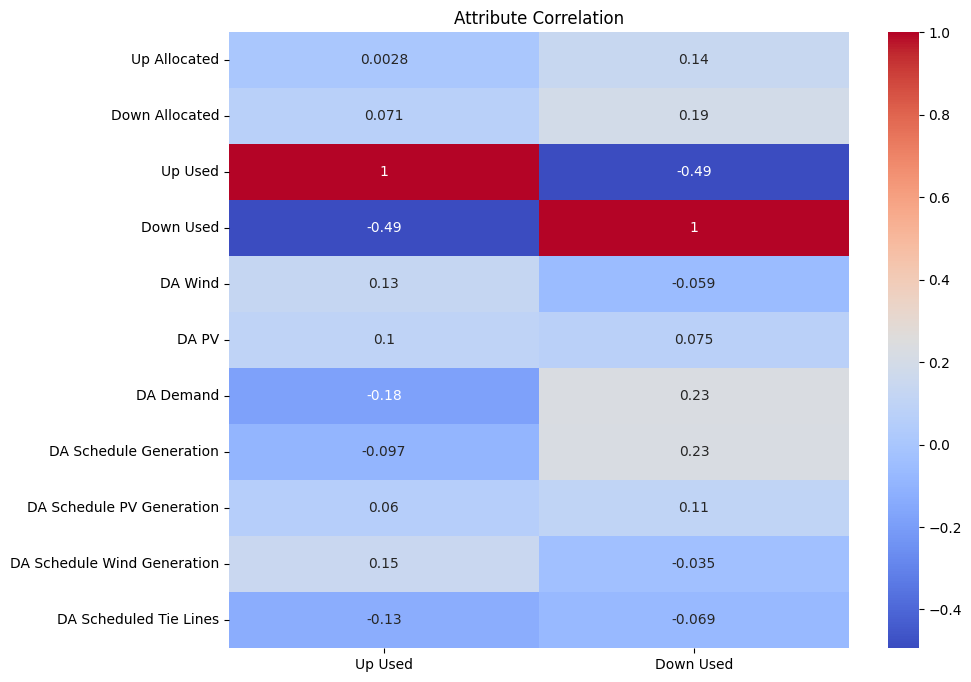
\includegraphics[width=\textwidth]{plots/correlation_heatmap.png}
    \caption{Attribute correlation}
    \label{fig:Attribute_correlation}
  \end{figure}
%   \unskip
  
 In Figure~\ref{fig:Attribute_correlation} is possible to verify that the correlation between allocated capacities and used energy is close to zero.  
  
The goal of this work is to reduce the difference between allocated capacities and used energy to efficiently use the available resources.

\subsubsection{Validation Data}
As for validation it was chosen the year 2024.\par
Using the non comparative metrics the results are presented in Table~\ref{validation_res}.

\begin{table}[H] 
    \caption{This is a table caption. Tables should be placed in the main text near to the first time they are~cited.\label{tab1}}
    \newcolumntype{C}{>{\centering\arraybackslash}X}
    \begin{tabularx}{\textwidth}{CCCCC}
    \toprule
    & \textbf{RMSE}	& \textbf{SAE}	& \textbf{AllocF} & \textbf{AllocD}\\
    \midrule
    Up Allocation (MW) & 536.55 & 17357826.75 & 152679.00 & 17205147.75 \\
    Down Allocation (MW) & 408.99 & 12981575.55 & 479191.60 & 12502383.95 \\
        \bottomrule
    \end{tabularx}
    % \noindent{\footnotesize{\textsuperscript{1} Tables may have a footer.}}
\end{table}



Table~\ref{validation_res} presents the main problems of the actual capacity allocation methodology, resulting with high: i) errors (RMSE and SAE) with used energy, ii) missing energy (AllocM), and iii) extra energy (AllocS).

The correlation between allocated energy in the current method to the used energy can be seen in Figure~\ref{fig:Attribute_correlation_benchmark}.

\begin{figure}[H]
    \centering
    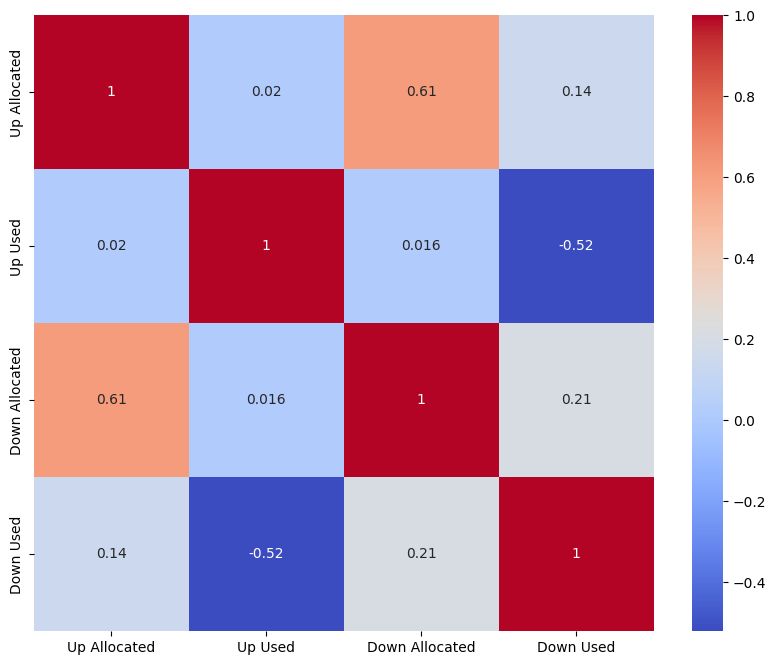
\includegraphics[width=0.75\textwidth]{plots/correlation_heatmap_benchmark.png}
    \caption{Attribute correlation benchmark}
    \label{fig:Attribute_correlation_benchmark}
  \end{figure}
%   \unskip

In Figure~\ref{fig:Attribute_correlation_benchmark} can be verified a high correlation between up and down allocated capacities, identifying the practically symmetrical used allocation.
%
Furthermore, the correlation of allocated capacities with used energy is small, which can be solved by using dynamic allocation as presented in the next section.

\subsection{Results}

The best results, only based on PPG Positive, for each architecture are presented in Tables~\ref{res_linear_forecast} and \ref{res_comparative_forecast}, were Vanilla means it is only one layer deep, and Stacked means two layers deep:

\begin{tabular}{llrrrrrrrrr}
\toprule
 &  & RMSE & SAE & AllocF & AllocD & GPD & GPD F & GPD D & GPD norm & GPD Positivo \\
 & Arquitetura &  &  &  &  &  &  &  &  &  \\
\midrule
\multirow[t]{5}{*}{Alocação a Subir} & UNET200 & 317.86 & 9759154.87 & 151181.25 & 9607973.62 & 43.78 & 0.98 & 44.16 & 22.57 & 43.78 \\
 & VanillaCNN200 & 328.88 & 10208138.49 & 147549.10 & 10060589.40 & 41.19 & 3.36 & 41.53 & 22.44 & 41.19 \\
 & UNET & 349.91 & 11008787.25 & 146742.39 & 10862044.86 & 36.58 & 3.89 & 36.87 & 20.38 & 36.58 \\
 & VanillaCNN & 370.73 & 11804382.23 & 149719.91 & 11654662.32 & 31.99 & 1.94 & 32.26 & 17.10 & 31.99 \\
 & 2StackedCNN200 & 410.28 & 13223932.55 & 126341.23 & 13097591.32 & 23.82 & 17.25 & 23.87 & 20.56 & 23.82 \\
\cline{1-11}
\multirow[t]{5}{*}{Alocação a Descer} & UNET200 & 282.52 & 8243468.87 & 469060.52 & 7774408.35 & 36.50 & 2.11 & 37.82 & 19.97 & 36.50 \\
 & VanillaCNN200 & 289.59 & 8671975.58 & 476040.73 & 8195934.85 & 33.20 & 0.66 & 34.45 & 17.55 & 33.20 \\
 & UNET & 304.28 & 9172373.23 & 470149.87 & 8702223.36 & 29.34 & 1.89 & 30.40 & 16.14 & 29.34 \\
 & VanillaCNN & 313.42 & 9483287.93 & 475881.60 & 9007406.33 & 26.95 & 0.69 & 27.95 & 14.32 & 26.95 \\
 & VanillaFCNN200 & 344.05 & 10438899.42 & 476740.17 & 9962159.25 & 19.59 & 0.51 & 20.32 & 10.41 & 19.59 \\
\cline{1-11}
\bottomrule
\end{tabular}


To choose the best model there was some analysis on \gls{PPG} and the individuals \gls{PPGS} and \gls{PPGM}. So that the final results would not just be the one best across the validation time, but also meanwise in the same time.\par
Regarding all variables in Table~\ref{training_vars} the chosen models can be described as presented in Table~\ref{chosen_models}.
\begin{table}[H] 
    \caption{Best Model Variable Description \label{chosen_models}}
    \newcolumntype{C}{>{\centering\arraybackslash}X}
    \begin{tabularx}{\textwidth}{CCCCCC}
    \toprule
    & \textbf{Architecture}	& \textbf{Advance Loss function ratio} & \textbf{Loss function} & \textbf{Activation} & \textbf{Weights}\\
    \midrule
    Up Allocation & StackedFCNN & 0.23 & MSE & ReLU & Mean \\
    Down Allocation & StackedFCNN & 0.002 & MSE & ReLU & Mean \\
        \bottomrule
    \end{tabularx}
    % \noindent{\footnotesize{\textsuperscript{1} Tables may have a footer.}}
\end{table}

Within the validation time, best model results can be summarized by Tables~\ref{pred_res_linear} and \ref{pred_res}:

\begin{table}[H] 
    \caption{Model Metric Results for Predictions. \label{pred_res_linear}}
    \newcolumntype{C}{>{\centering\arraybackslash}X}
    \begin{tabularx}{\textwidth}{CCCCC}
    \toprule
    & \textbf{RMSE}	& \textbf{SAE}	& \textbf{AllocM} & \textbf{AllocS}\\
    \midrule
    Up Allocation (MW) & 570.21 & 4506080.04 & 40569.85 & 4465510.18 \\
    Down Allocation (MW) & 694.80 & 5811536.58 & 13619.08 & 5797917.50 \\
        \bottomrule
    \end{tabularx}
    % \noindent{\footnotesize{\textsuperscript{1} Tables may have a footer.}}
\end{table}


\begin{table}[H] 
    \caption{Model/Benchmark Comparative Metrics Results for predictions. \label{pred_res}}
    \newcolumntype{C}{>{\centering\arraybackslash}X}
    \begin{tabularx}{\textwidth}{CCCCC}
    \toprule
    & \textbf{PPG}	& \textbf{PPG M}	& \textbf{PPG S} \\
    \midrule
    Up Allocation (\%) & 21.77 & 1.24 & 21.92 \\
    Down Allocation (\%) & 11.39 & 9.31 & 11.39 \\
        \bottomrule
    \end{tabularx}
    % \noindent{\footnotesize{\textsuperscript{1} Tables may have a footer.}}
\end{table}



With an overall description as follows in Table~\ref{model_vs_bench}:
% meter tableas dos resutlados com benchmark
\begin{table}[H] 
    \caption{Model Results and (allocated) values wthin 2024.\label{model_vs_bench}}
    \begin{adjustwidth}{-\extralength}{0cm}
    \newcolumntype{C}{>{\centering\arraybackslash}X}
    \begin{tabularx}{\fulllength}{CCCCCC}
    \toprule
    & & \textbf{mean}	& \textbf{std}	& \textbf{min} & \textbf{max}\\


    \midrule
            \multirow[m]{2}{*}{Down Allocation (MW)}	        & & (921.84) & (191.03) & (720.00) & (1708.00) \\
                                                                & & 836.85 & 182.04 & 247.82 & 1469.62 \\
            \multirow[m]{2}{*}{Up Allocation (MW)}	            & & (921.49) & (191.72) & (719.00) & (1694.00) \\
                                                                & & 778.42 & 228.85 & -29.47 & 1458.01 \\
            \multirow[m]{2}{*}{Hourly Capacity (MW)}	        & & (1843.32) & (382.35) & (1439.00) & (3399.00) \\
                                                                & & 1615.27 & 346.50 & 393.85 & 2594.85 \\
            \multirow[m]{2}{*}{Extraordinary Down Energy (MWh)}	& & (168.74) & (175.69) & (0.90) & (1214.00) \\
                                                                & & 149.66 & 179.96 & 2.66 & 1358.81 \\   
            \multirow[m]{2}{*}{Extraordinary Up Energy (MWh)}	& & (179.39) & (163.94) & (1.00) & (1054.80) \\
                                                                & & 141.85 & 153.57 & 1.83 & 1420.22 \\
    \bottomrule
    \end{tabularx}
    \end{adjustwidth}
\end{table}


The proposed model presents an overall improvement of \textasciitilde22\% in upward allocation and \textasciitilde11\% in downward allocation, comparing to current allocation methods.\par
Where the hourly means differences between benchmark and validation results are presented in Table~\ref{model_vs_bench_perc}.

% meter tableas dos resutlados dos deltas com benchmark
\begin{table}[H] 
    \caption{Mean $\Delta$\% between model and benchmark\label{model_vs_bench_perc}}
    \newcolumntype{C}{>{\centering\arraybackslash}X}
    \begin{tabularx}{\textwidth}{CC}
    \toprule
    & \textbf{$\Delta$\%} \\
    

    \midrule
            Down Allocation (MW)	        & -28.62 \\
            Up Allocation (MW)              & -37.26 \\
            Hourly Capacity (MW)	        & -33.24 \\
            Extraordinary Down Energy (MWh)	& -51.62 \\
            Extraordinary Up Energy (MWh)	& -59.47 \\
    \bottomrule
    \end{tabularx}
    % \noindent{\footnotesize{\textsuperscript{1} Tables may have a footer.}}
\end{table}




Average hourly improvements are of \textasciitilde16\% and \textasciitilde9\% respectively, which also is an improvement on state of the art \cite{Algarvio2024} with 13\% and 8\%.
The current study can free in average \textasciitilde12\% of hourly resources, lowering the need to allocate down and up capacity to the secondary reserve in \textasciitilde21\% and \textasciitilde11\%, respectively.\par

Can also be checked that the correlation between used and alocated is bigger than in the current method, achieving 36\% in both upward energy and downward energy. \par

\begin{figure}[H]
    \centering
    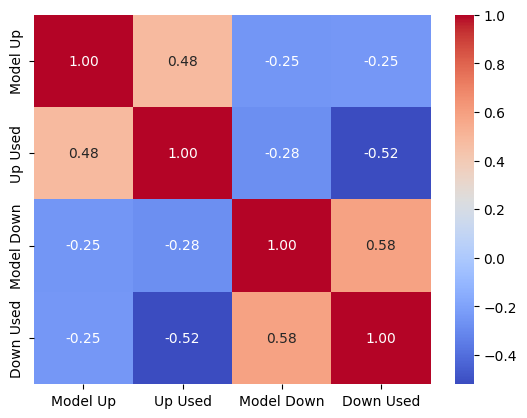
\includegraphics[width=0.75\textwidth]{plots/heatmap_correlation_pred.png}
    \caption{Attribute correlation}
    \label{fig:Attribute_correlation}
  \end{figure}


 \par

% The proposed dynamic reserve procurement methodology is implemented in three main steps:

% \subsubsection*{Forecasting Reserve Needs}
% Machine learning models are trained to predict the upward and downward reserve requirements based on day-ahead forecasts of vRES generation and system demand. Models such as Long Short-Term Memory (LSTM) networks, Random Forests, and XGBoost are used to capture temporal and nonlinear dependencies in the data. The inputs to the models include historical forecasts, real-time deviations, and weather data.

% \subsubsection*{Dynamic Allocation of Reserves}
% Using the machine learning forecasts, the required reserve capacities are dynamically adjusted for upward and downward reserves. The allocation considers real-time deviations observed in previous periods and adjusts procurement to better match actual system needs.

% \subsubsection*{Performance Evaluation}
% The performance of the dynamic reserve procurement is evaluated using key metrics, including:
% \begin{itemize}
%     \item \textbf{Forecast Error (RMSE and MAE)}: Measures the accuracy of reserve predictions.
%     \item \textbf{Reserve Utilization Rate}: Assesses the alignment between procured and activated reserves.
%     \item \textbf{Cost Efficiency}: Compares the costs of dynamic procurement with traditional static methods.
% \end{itemize}

% \subsection*{Results and Analysis}
% The results of the case study demonstrate significant improvements in reserve allocation efficiency compared to the traditional static methods currently used by the Spanish TSO.

% \subsubsection*{Forecast Accuracy}
% The machine learning models, particularly the LSTM network, outperformed traditional statistical methods such as ARIMA in predicting reserve requirements. The Root Mean Square Error (RMSE) was reduced by 15-20\% for both upward and downward reserve predictions.

% Incorporating weather variables into the models significantly improved the accuracy of vRES generation forecasts, which directly influenced reserve predictions.

% \subsubsection*{Reserve Utilization}
% The dynamic approach led to a higher utilization rate of procured reserves. The proportion of unused reserves was reduced by approximately 10\%, indicating a better alignment between forecasted and actual reserve needs.

% Asymmetrical reserve procurement allowed for flexibility in addressing specific system needs, such as prioritizing downward reserves during periods of high solar generation.

% \subsubsection*{Cost Efficiency}
% The dynamic procurement methodology reduced total reserve procurement costs by 8-12\% compared to static allocation methods. This cost savings was primarily driven by the reduction in over-procurement of reserves.

% The analysis showed that the optimized reserve allocation minimized the activation of expensive balancing reserves in the real-time market, further improving cost efficiency.

% \subsubsection*{Impact of vRES Penetration}
% The benefits of dynamic procurement were more pronounced during periods of high vRES penetration, where forecast uncertainty and variability were greatest. This highlights the importance of adapting reserve allocation methodologies to accommodate the increasing share of renewable generation.
